\section{Data Methodology within UniTraj}
\label{sec:data_methodology}

This section presents the data processing methodology within the UniTraj framework~\cite{unitrajFeng2024}, covering the transformation from heterogeneous autonomous driving datasets to standardized tensor representations suitable for trajectory prediction models. UniTraj serves as a unified interface that harmonizes datasets from WOMD~\cite{WOMD2021}, Argoverse2~\cite{av2Wilson2023}, and nuScenes~\cite{caesar2020nuscenes} through the ScenarioNet format~\cite{scenarionetLi2023}.

\subsection{UniTraj's Data Processing Pipeline}
\label{ssec:data_pipeline}

The UniTraj preprocessing pipeline transforms raw, heterogeneous data into standardized, model-ready tensors through a multi-phase process. Each phase is implemented as a distinct method within the \texttt{DataParser} class, ensuring modularity and clarity. The following provides a brief qualitative overview of the pipeline; for detailed implementations and more comprehensive descriptions, see ~\autoref{app:framework}.

\begin{description}
    \item[Phase 1: Temporal Window Extraction] Extracts fixed-length time windows from raw trajectories and applies frequency masking for uniform temporal sampling (\autoref{alg:phase1_temporal}).
    \item[Phase 2: Map Feature Processing] Converts raw map data (lanes, boundaries) into standardized polylines with uniform point density and semantic encodings (\autoref{alg:phase2_map}).
    \item[Phase 3: Agent Selection] Filters for relevant agents based on motion and observation quality to identify suitable prediction candidates (\autoref{alg:phase3_filtering}).
    \item[Phase 4: Coordinate Transformation] Transforms the entire scene into an agent-centric coordinate frame for each candidate, ensuring translation and rotation invariance (\autoref{alg:phase4_transform}).
    \item[Phase 5: Feature Assembly] Constructs comprehensive feature vectors for each agent, concatenating spatial, kinematic, and semantic attributes (\autoref{alg:phase5_features}).
    \item[Phase 6: Proximity Filtering \& Padding] Selects the \(N_{\max}\) closest agents and pads the agent tensor to a fixed size for batching (\autoref{alg:phase6_proximity}).
    \item[Phase 7: Map Tensorization] Segments, resamples, and selects the \(K_{\max}\) closest map polylines, creating a fixed-size map tensor (\autoref{alg:phase7_map_features}).
    \item[Phase 8: Future Processing] Processes and transforms the ground truth future trajectories for the center agent (\autoref{alg:phase8_future}).
    \item[Phase 9: DatasetItem Assembly] Assembles all processed tensors and masks into a final \texttt{DatasetItem}, the fundamental unit of the dataset (\autoref{alg:phase9_assembly}).
\end{description}

\paragraph{The \texttt{BaseDataParser} Class.}
The \texttt{BaseDataParser} serves as the central orchestrator of the data processing pipeline. It coordinates the parallel processing of scenario chunks, manages HDF5 file storage of the resulting dataset, and assembles the metadata that is collected throughout the pipeline.\\

\subsection{The UniTraj DatasetItem and Batching}
\label{ssec:unitraj_dataset}

The output of the processing pipeline is a collection of \texttt{DatasetItem} instances, each encapsulating a complete prediction scenario in a standardized format.

\paragraph{The \texttt{DatasetItem} Structure.}
A \texttt{DatasetItem} is a strongly typed object that holds all the \texttt{numpy} arrays corresponding to a single, agent-centric view of a scene. This includes the historical agent states, the map geometry, ground truth future trajectories, and associated validity masks. The \texttt{DatasetItem} contains all necessary data for training, evaluation, analysis and visualization, and hence contains many redundant features.

\paragraph{Batching with the \texttt{collate\_fn}.}
For model training and inference, individual \texttt{DatasetItem}s are grouped into batches by a PyTorch \texttt{DataLoader} within a \texttt{pl.DataModule}. This process is orchestrated by a custom \texttt{collate\_fn}, which transforms a list of \texttt{DatasetItem}s into a typed dictionary of tensors which can subsequently be used as model input.

The key tensors within this batch structure are described below. For complete tensor specifications, dimensions, and feature breakdowns, refer to Tables~\ref{tab:data_tensors},~\ref{tab:agent_types}, and~\ref{tab:polyline-types} in \autoref{app:notation}.

\paragraph{Dynamic Agent Representation.}
Agent trajectories are encoded in tensor \(\boldsymbol{X}_d \in \mathbb{R}^{B \times N_{\max} \times T_p \times F_{ap}}\), where \(B\) is the batch size. It contains comprehensive state information for up to \(N_{\max}\) agents over \(T_p\) historical timesteps. The agent feature dimension \(F_{ap}\) encompasses spatial coordinates, physical dimensions, one-hot encoded object types, temporal position embeddings, heading, and kinematic states. The corresponding validity mask \(\boldsymbol{M}_d \in \{0,1\}^{B \times N_{\max} \times T_p}\) indicates data availability.

\paragraph{Static Map Representation.}
High-definition map information is represented through tensor \(\boldsymbol{X}_s \in \mathbb{R}^{B \times K_{\max} \times L \times F_{map}}\), encoding up to \(K_{\max}\) polylines with \(L\) points each. The \(F_{map}\) features capture geometric and semantic properties, including polyline point coordinates, direction vectors, and lane type classifications. The validity mask \(\boldsymbol{M}_s \in \{0,1\}^{B \times K_{\max} \times L}\) handles variable map complexity.

\paragraph{Ground Truth and Auxiliary Data.}
Future trajectory targets for the center agent are provided in \(\boldsymbol{y}_c \in \mathbb{R}^{B \times T_f \times F_{af}}\), where \(F_{af}\) includes position and velocity over \(T_f\) prediction timesteps. The batch also contains metadata like Kalman-difficulty scores and classifications of the type of maneuver that the center agent is performing.

\paragraph{Sample Metadata and Dataset Composition.}
UniTraj maintains metadata for efficient dataset management and analysis. The sample metadata, stored as a pandas DataFrame that provides high-level information about each scenaro. Each entry is uniquely identified by a composite index encoding the dataset name, worker process, scenario counter, and agent index (e.g., \texttt{av2\_scenarionet{-}0{-}0{-}0}). A complete overview of the sample metadata fields is provided in Table~\ref{tab:sample_metadata_fields}.

\paragraph{DatasetItem Visualization.}
To illustrate the comprehensive nature of the processed data, Figure~\ref{fig:datasetitem_visualization} presents a detailed visualization of a representative \texttt{DatasetItem}. This enhanced visualization demonstrates the multi-modal nature of the data, showing the spatial relationships between agents, their historical trajectories, and the underlying high-definition map infrastructure.

\begin{figure}[htbp]
    \centering
    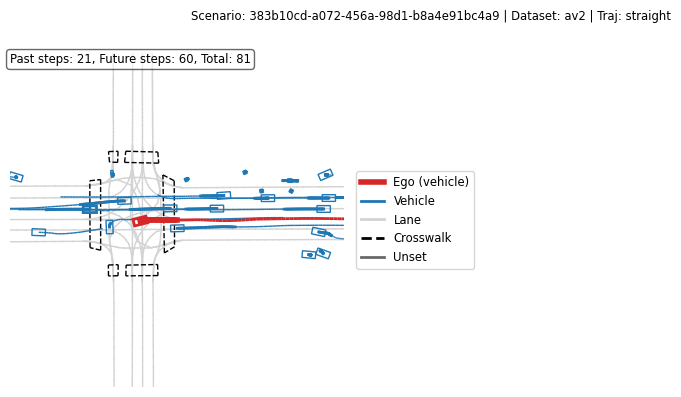
\includegraphics[width=\textwidth]{figures/plot_datasetitem.png}
    \caption{
        \textbf{Enhanced DatasetItem Visualization.} A comprehensive view of a processed scenario showing: (a) the center agent (ego vehicle) in red with its historical trajectory, (b) surrounding agents with their temporal information including velocity vectors and heading indicators, (c) high-definition map polylines with semantic classifications (lanes in blue, crosswalks in black dashed, boundaries in gray), and (d) agent interaction zones and proximity relationships. This visualization demonstrates the multi-modal nature of the standardized \texttt{DatasetItem} format, capturing spatial and temporal dynamics used for trajectory prediction tasks.
    }
    \label{fig:datasetitem_visualization}
\end{figure}

\newpage